\documentclass[prb,preprint]{revtex4-1} 

\usepackage{amsmath}  
\usepackage{amsfonts} 
\usepackage{graphicx} 
\usepackage{gensymb}
\usepackage{enumerate}

\begin{document}

\title{Measurement of Faraday Rotation and Calculation of the Verdet Constant for a SF-59 Glass Rod}

\author{Frances Yang}
\email{fyang@smith.edu} 

\author{Isabel Lipartito}
\email{iliparti@smith.edu}
\affiliation{Department of Physics, Smith College, Northampton, MA 01063}

\date{\today}

\begin{abstract}
{We observed the Faraday effect, a shift in the polarization of light as it passes through medium subject to a magnetic field. Polarized light from a 650 nm laser was sent through a SF-59 glass rod surrounded by a solenoid. The light then passed through an rotatable polarizer and was detected by a photodiode. We calculated the Verdet constant for the rod by varying the magnetic fields and measuring the relative polarization shift and the voltage shift at a particular polarizer angle. From two separate calculations, we found a Verdet constant of $19.9 \pm 1.0 \mathrm{~rad/T} \cdot \textrm{m}$ and $17.54 \pm 1.12 \mathrm{~rad/T} \cdot \textrm{m}$. Other colleagues performing the experiment found the Verdet constant to be between 19 and 23$\mathrm{~rad/T} \cdot \textrm{m}$ from using the first method and between 19 and 21$\mathrm{~rad/T} \cdot \textrm{m}$ from using the second method.  In our paper, we address a possible systematic error that lead to our Verdet constant being too low from the second method.

}
\end{abstract}

\maketitle 
\section{Aims}
{
\begin{enumerate}[(a)]
\item To demonstrate the Faraday effect of the rotation of the plane of polarization of light as it travels through magnetic fields of different magnitudes.

\item To calculate the Verdet constant ($V_{c}$) relating the change in polarization angle to the change in magnetic field.
\begin{equation}
\label{vconst}
\Delta \phi =V_{c}\hspace{1.5pt} \Delta B\hspace{1pt}\textrm{L}{_{\textrm{sample}}}
\end{equation}
\end{enumerate}
}
\section{Introduction} 

{The Faraday effect is a magneto-optical phenomenon in which light of a single wavelength, traveling through certain materials subject to a magnetic field, experiences a shift in the plane of polarization. These materials, called birefringent, have different refractive indices for the right and left circular polarizations of light. As light travels through the material, the relative phase angle between the two polarizations changes, rotating the overall polarization plane \cite{melissinos}.  

The Faraday effect was discovered by Michael Faraday in 1845 and was the first experimental demonstration of the interrelation of electricity and magnetism.  It has a strong historical significance and is a benchmark in the development of electromagnetic theory \cite{melissinos}.  It also is of primary importance in many contemporary research fields in physics.  For example, the Faraday Effect is currently being used to probe the properties of systems of interacting quantum spins, or spin-liquids.\cite{spin}


As shown in Eq.~(\ref{vconst}) , $V_{c}$ is a constant of proportionality that relates the change in polarization angle to the change in the magnetic field.\cite{expphysics} The value of $V_{c}$ depends on the medium and the wavelength of the light. The intensity of the light is given by $I=I_{0}\cos^{2}(\theta)$, where $\theta$ is the polarization angle with respect to the angle of  maximum intensity. When light experiences the Faraday effect, there will be a shift in the polarization so the intensity will be given by $I=I_{0}*\cos^{2}(\theta+\phi)$ instead.
}

\section{Procedure}
{Polarized light came from a 650 nm laser, driven by a 400 kHZ square wave from a function generator. A 15.2 cm long solenoid with 1400 turns and a DC resistance of 1.6 $\Omega$ was the source of our magnetic field. The current for the solenoid was provided by a Keithley 2230-30-1 DC Power Supply. Channel 1 and Channel 2 were connected in parallel to provide sufficient current. The calibration of the solenoid was found by measuring the magnetic field at the center of the solenoid for a current of 0 A to 2.25 A in steps of 0.25 A. The calibration constant was calculated to be $10.6 \textrm{~mT/A} \pm 0.05 \text{~mT}$. A 10.2 $\pm$ 0.5 cm SF-59 glass rod, was centered inside the solenoid. SF-59 glass is a heavy flint glass of refractive index 1.95 \cite{optics}.  The light is passed through a polarizer and detected by a photodiode, with the setting at 1 k$\Omega$. The photodiode outputs a voltage signal proportional to the detected light intensity\cite{teachspin}. A diagram of the experimental setup is shown in Fig.~\ref{setup}.

\begin{figure}
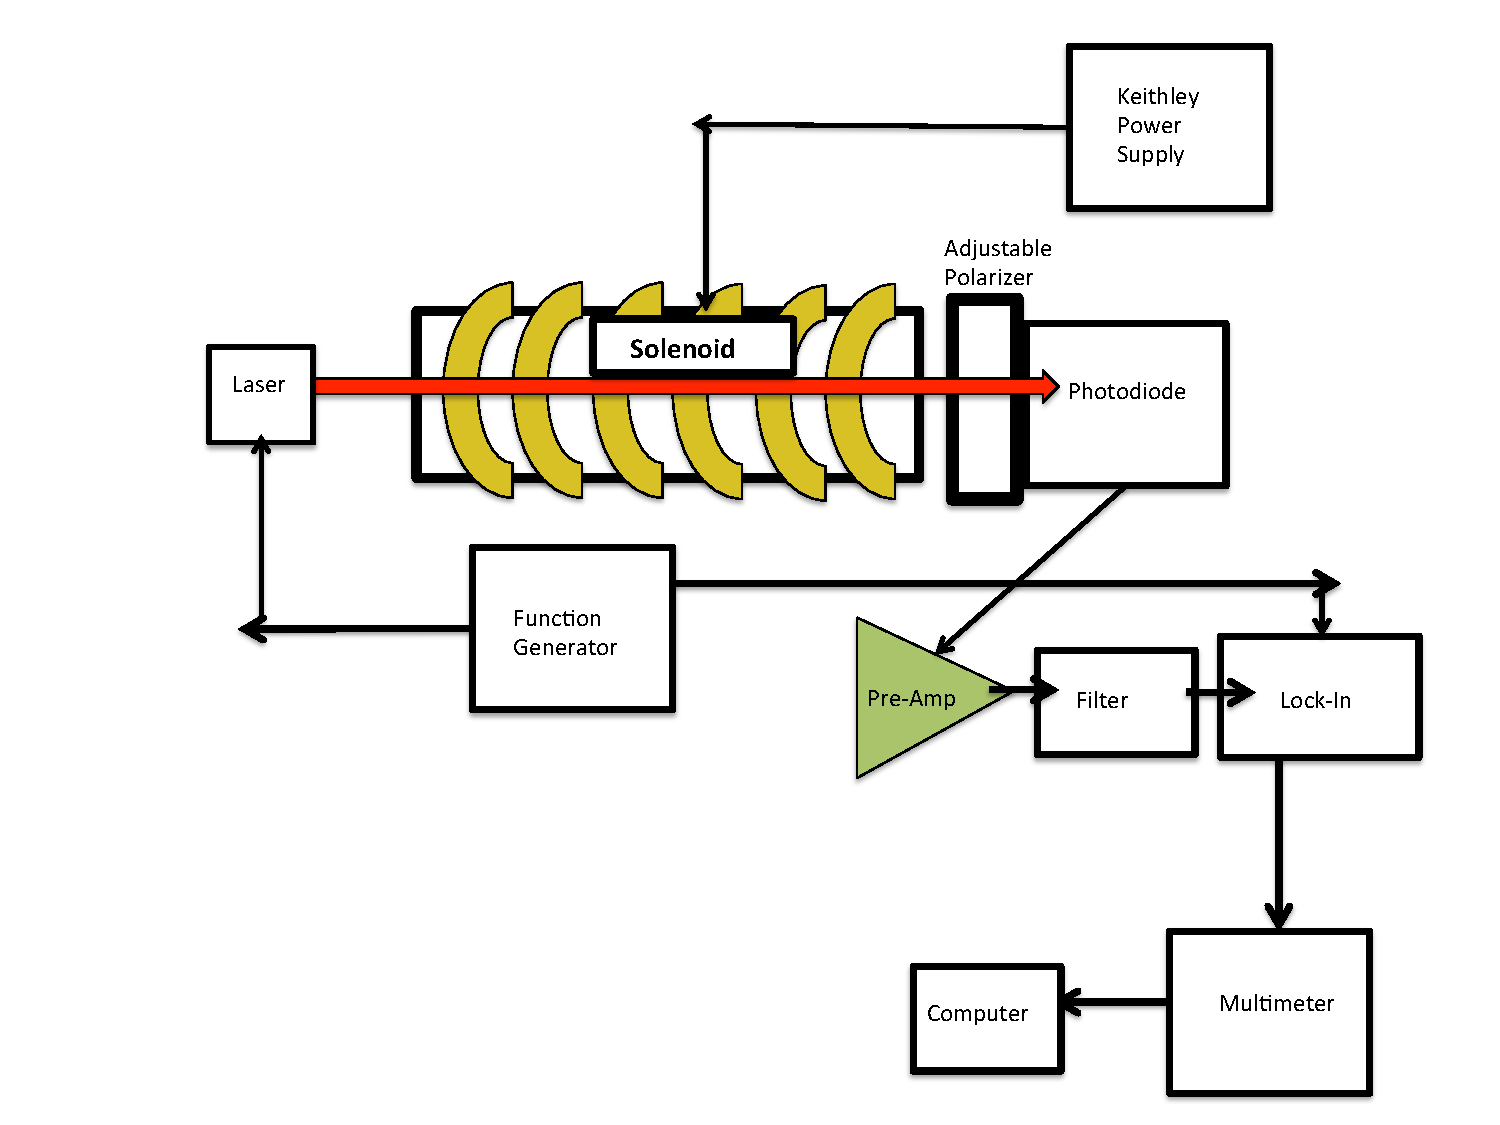
\includegraphics[width = 4.3in]{ExperimentalSetup}
\caption{\label{setup}A flow diagram of our experimental setup}
\end{figure}

A lock-in amplifier was used so undesirable noise such as light from the environment and drift from the photodiode, can be removed from the signal. The output of the photodiode was connected to a band pass filter with a center frequency of 400 kHz and a Q of 20. This extracted the first harmonic of the square wave, a 400 kHz sine wave. The output of of the filter was connected to a lock-in amplifier of gain 5. The reference signal for the lock-in amplifier was a 400 kHz sine wave with the same phase as the square wave driving the laser. It was generated by the same function generator for the square wave. The voltage output signal from the lock-in was measured by a Keithley 2100 Digital Multimeter.

Voltage readings from the multimeter were recorded onto the computer using LabView program (Keithley DC Incremental Write.vi). Each recorded voltage was an average of 16 measurements. We took two types of measurements, so the Verdet constant can be calculated in two ways.  The first method recorded the voltages as the polarizer was rotated in increments of 5\degree. We used this method with magnetic field values of -10.6 mT, 0 mT, 15.9 mT, and 21.2 mT. The negative field was generated by reversing the connection of the two leads of the power supply to the solenoid. The second method set the polarizer at an angle of $\theta = 45\degree$, as it is the most sensitve angle. The voltages at field values of $-31.8$--$31.8$ mT, in increments of $5.3$ mT were measured.
}


\section{Results}
{Figs.~\ref{nofield}--\ref{maxfield} show the voltages plotted against the polarizer angle for different magnetic field. Fig.~\ref{method1pic} shows the voltages measured at an angle of $\theta=45\degree$ for different magnetic fields. 
\begin{figure}[h]
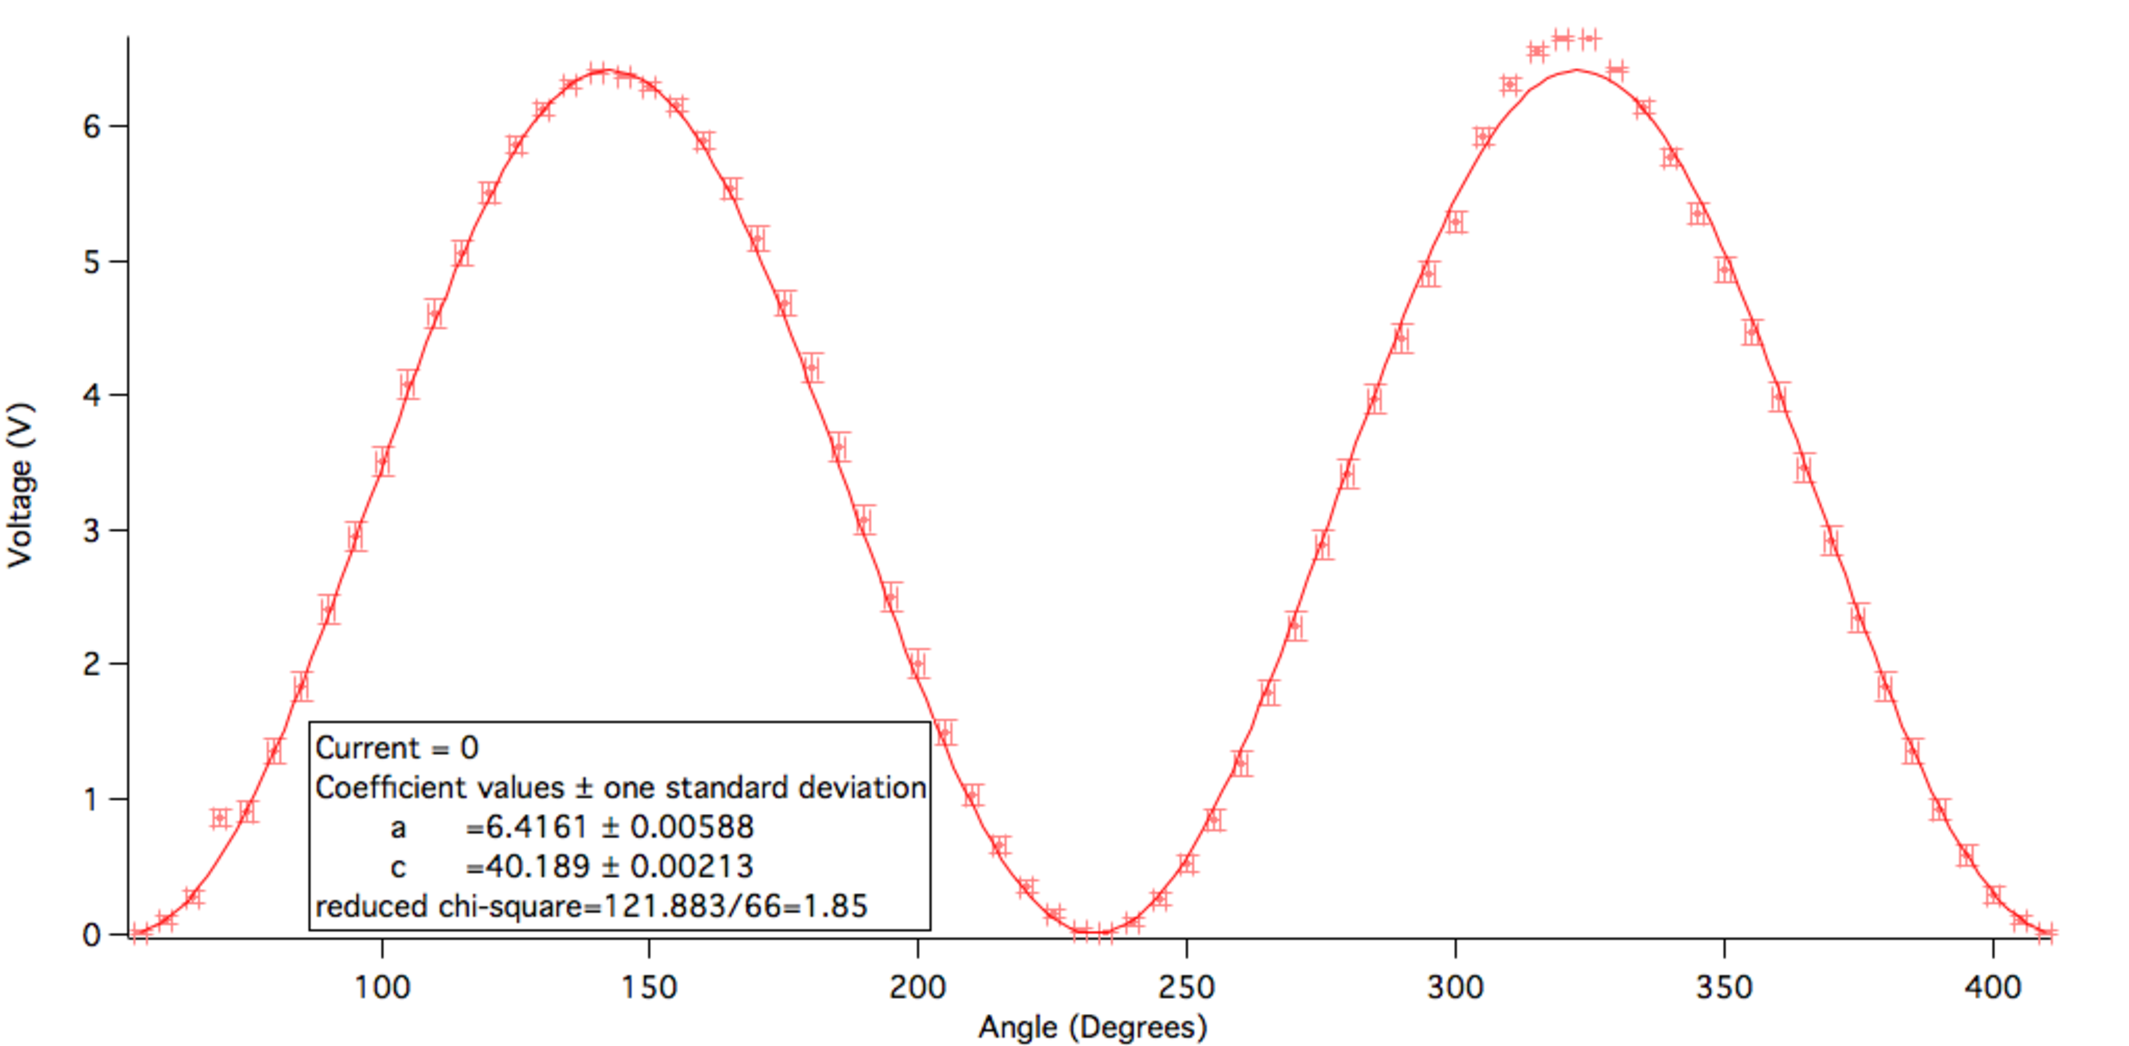
\includegraphics[width = 5.8in]{0A.pdf}
\caption{\label{nofield}Photodiode voltage measured for no magnetic field.}
\end{figure}

\begin{figure}
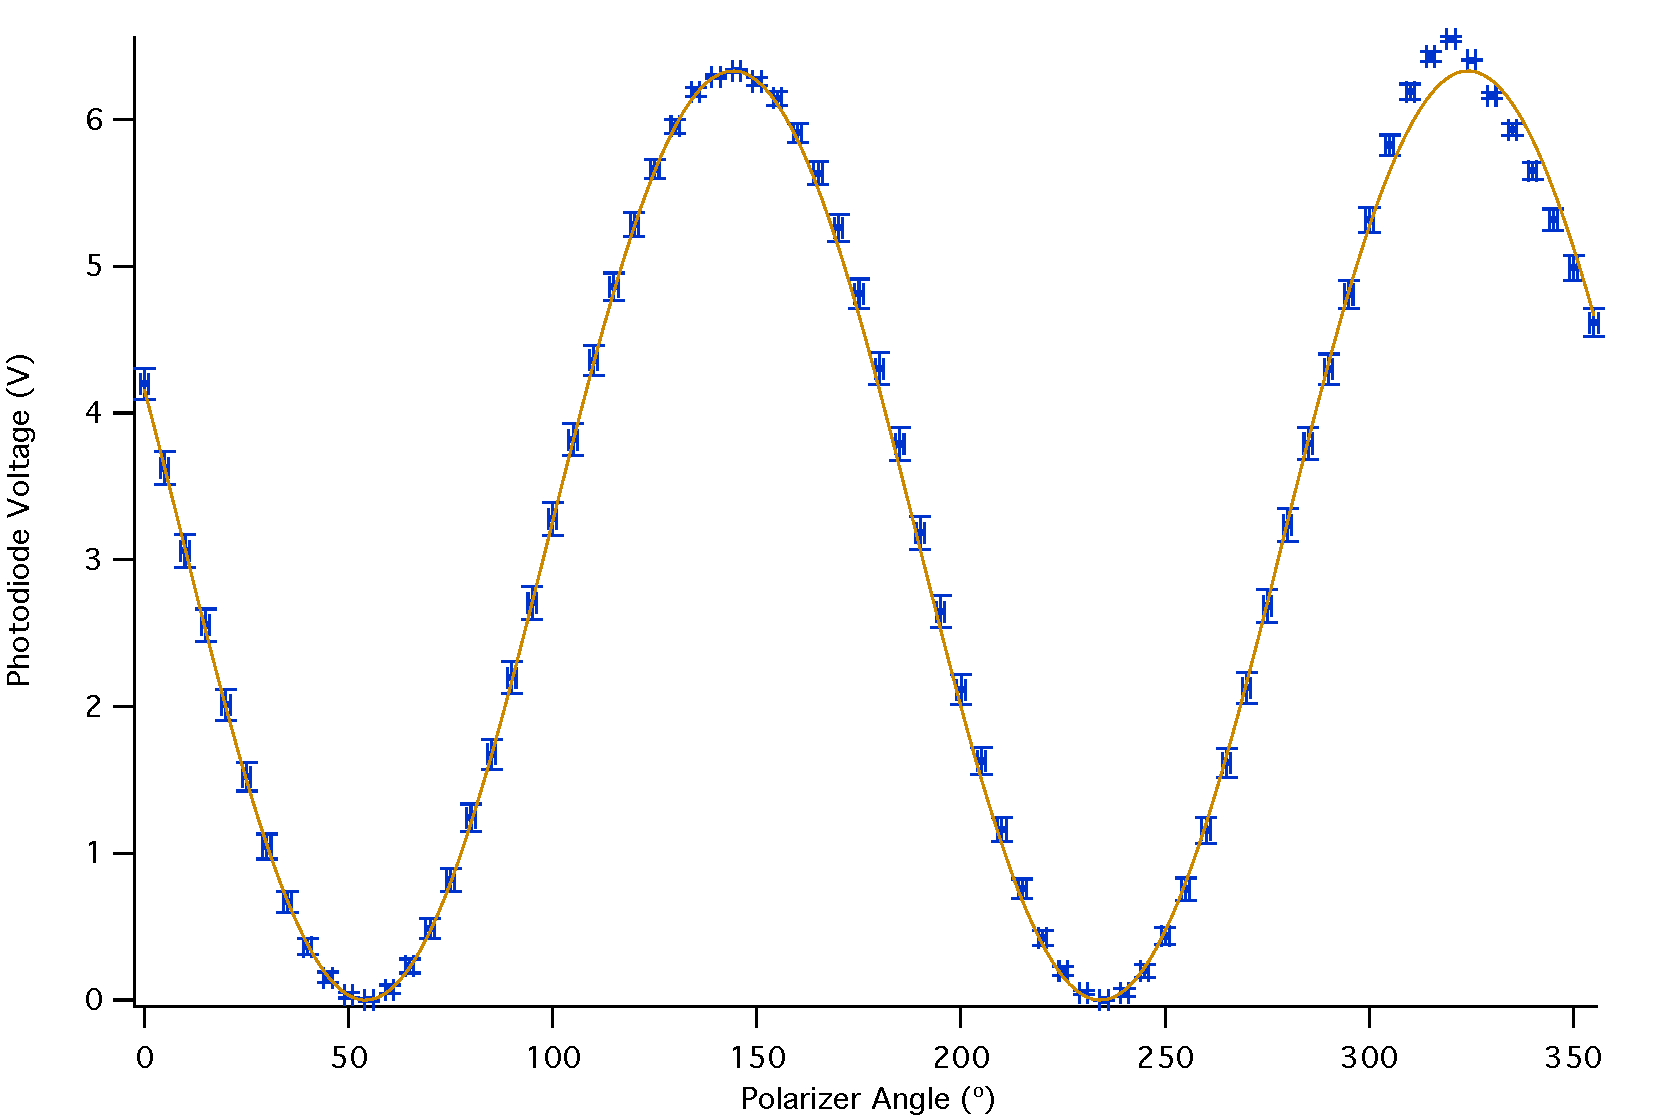
\includegraphics[width = 5.8in]{n1A.pdf}
\caption{\label{neg}Photodiode voltage measured for a magnetic field of -10.6 mT.}
\end{figure}

\begin{figure}
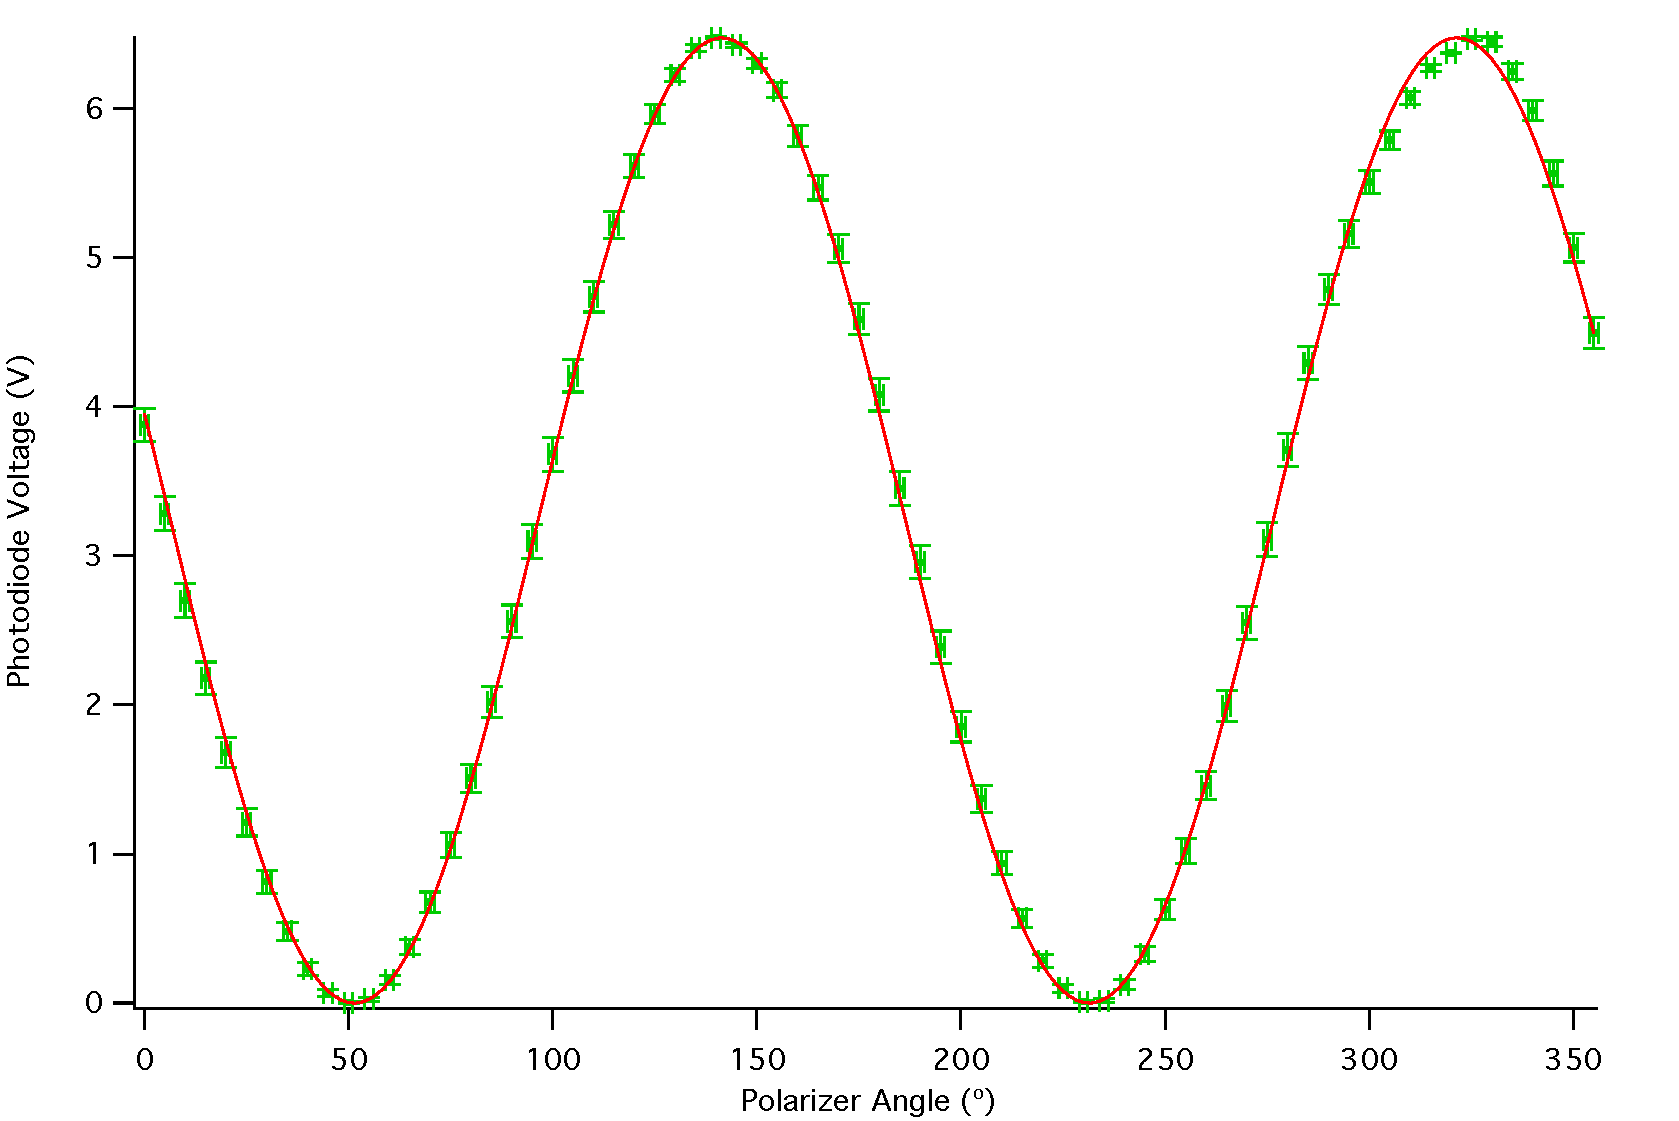
\includegraphics[width = 5.8in]{15A.pdf}
\caption{\label{onehalf}Photodiode voltage measured for a magnetic field of 15.9 mT.}
\end{figure}

\begin{figure}
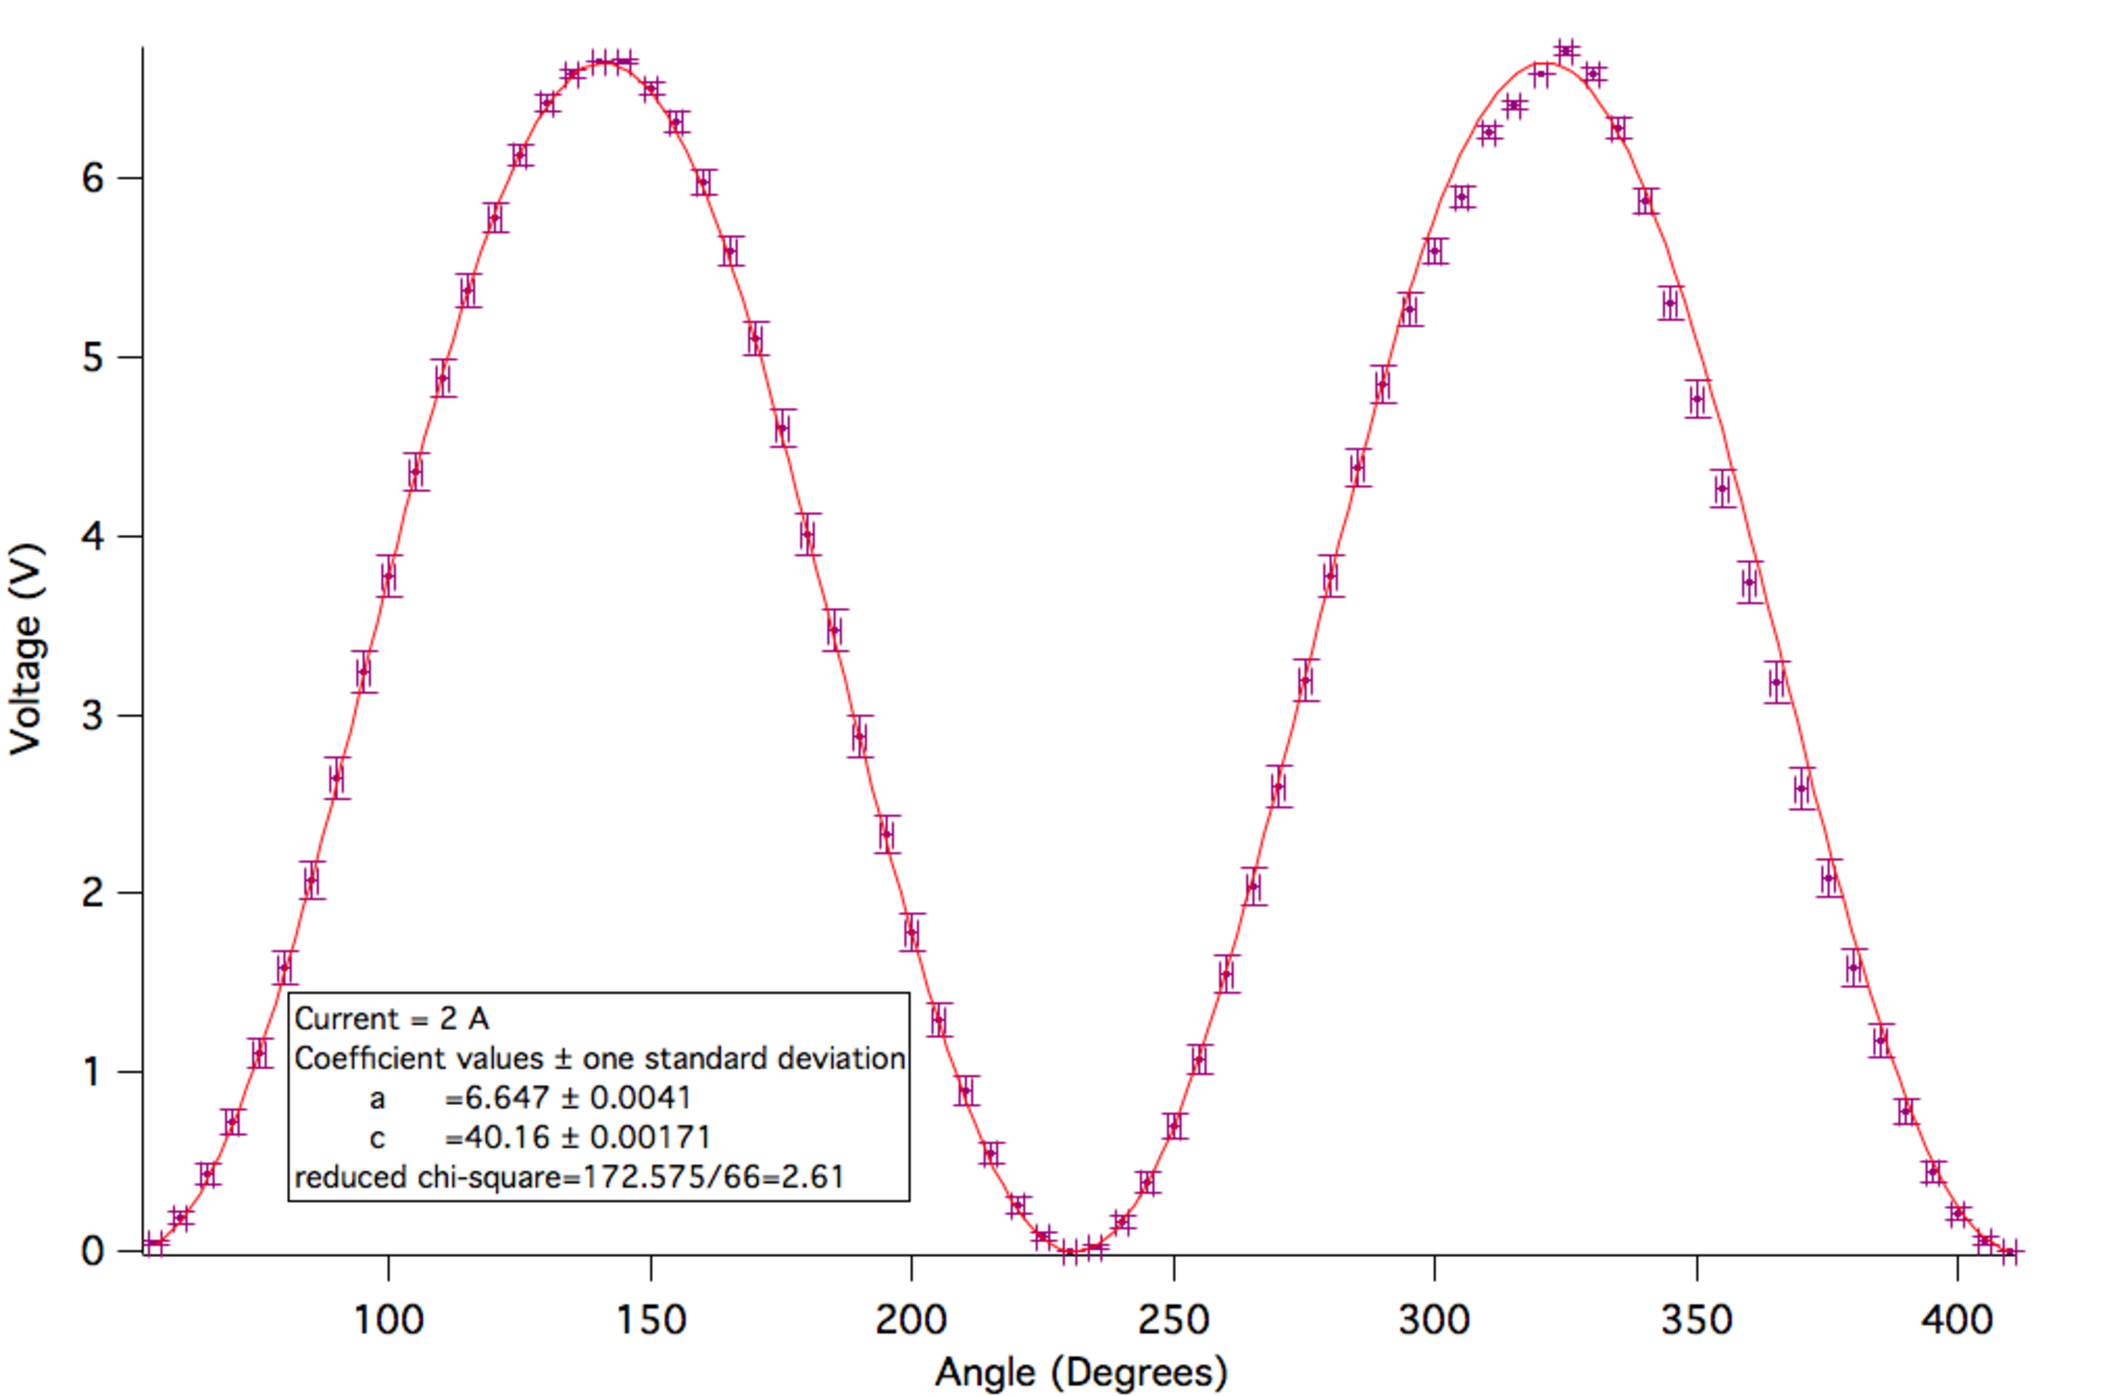
\includegraphics[width = 5.8in]{2A.pdf}
\caption{\label{maxfield}Photodiode voltage measured for a magnetic field of 21.2 mT.}
\end{figure}

\begin{figure}
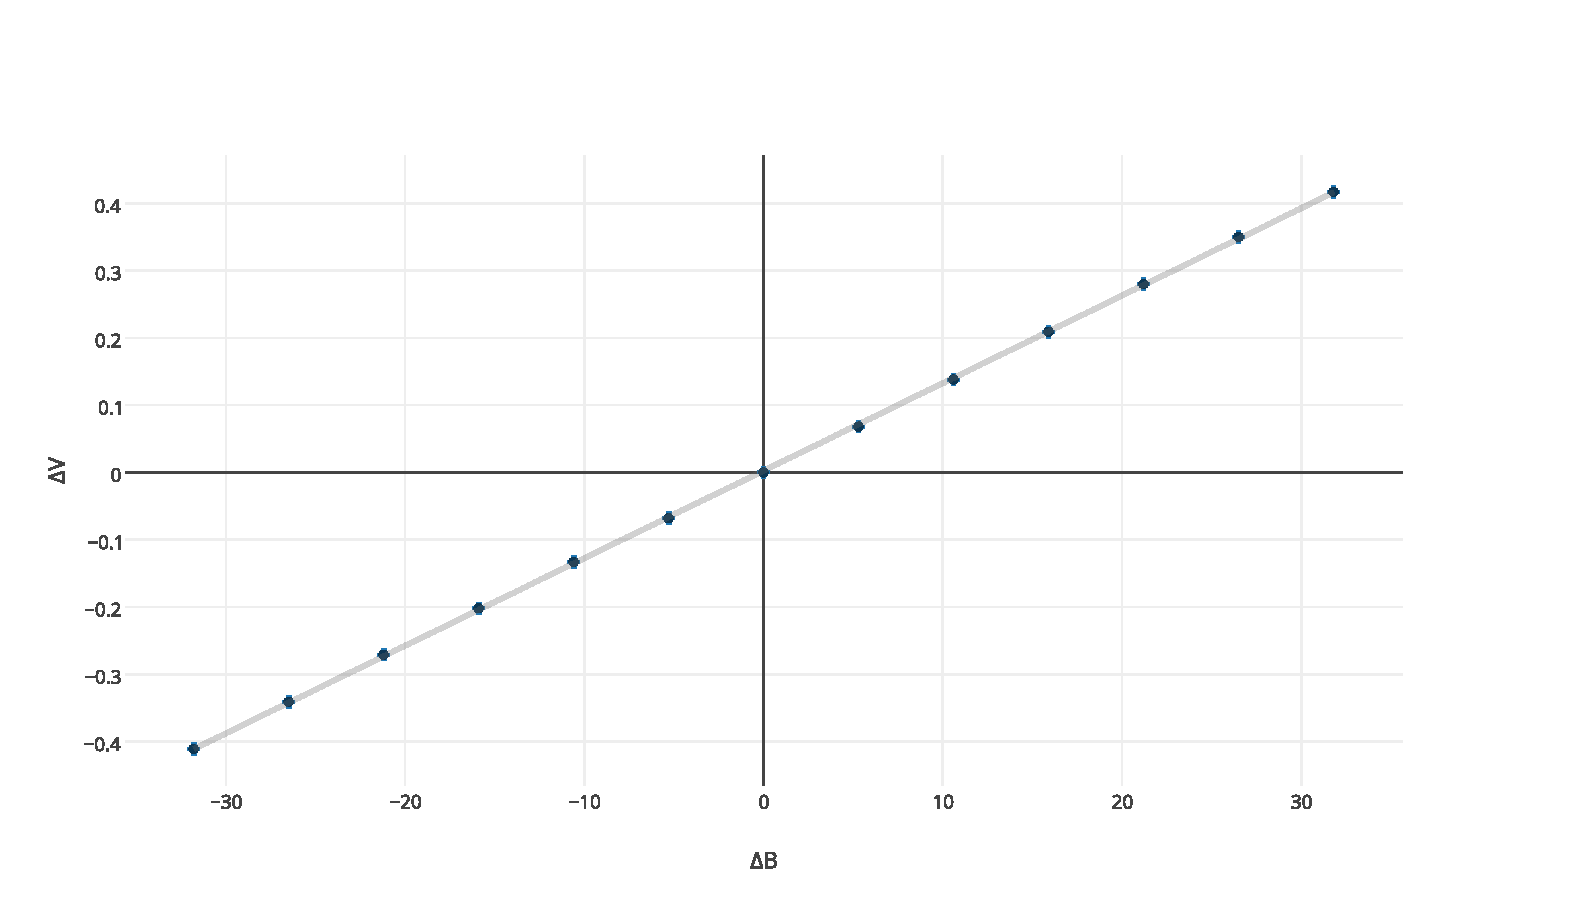
\includegraphics[width =6.3in]{verdetpic2.pdf}
\caption{\label{method1pic} The measured change in photodiode voltage for a change in the magnetic field at a polarizer angle 45\degree\  from the maximum voltage output. A linear fit was used to determine $\Delta V/\Delta B$.}
\end{figure}
}

\section{Analysis}
{\subsection{Method 1: Measurement of Photodiode Voltage for Various Polarizer Angles}
{A cosine-squared fit was performed on each our voltage measurements corresponding to a different a magnetic field. The curve fits are shown in Figs.~\ref{nofield}--\ref{maxfield}.  One point in the curve fit for the B=0 dataset was excluded from the curve fit because we measured the voltage twice for one angle. In all data sets, the experimental measurements of voltage for polarizer angles around 305\degree--340\degree were systematically higher than the values predicted by the sinusoidal curve fit. After a polarizer angle of 340\degree, we noticed that our experimental data values began to agree once again with the sinusoidal fit.  In the Discussion section, we discuss possible causes for this systematic error. We masked the values corresponding to angles of 305\degree--340\degree\ (305\degree--330\degree) were masked from the curve fits as well for datasets with a nonzero magnetic field (no magnetic field) so they would not skew our calculation of the Verdet constant.

Our dominant source of error in these measurements is from setting the polarizer at the correct angle. We were able to set the polarizer within $1\degree$ of the desired angle. This error in the polarizer angle was propagated to an error in the voltage. We neglected voltage error from the multimeter as it was many magnitudes smaller than the error due to the angle.

The results of the curve fits are listed in Table~\ref{shift table}. We plotted $\Delta \phi$ agains $\Delta B$ in Fig.~\ref{method1pic}. A linear fit was performed to to obtain $\Delta \phi/\Delta B=1.79 \pm 0.07\textrm{~rad/T}$. The Verdet constant was calculated by rearranging Eq.~(\ref{vconst}) to
\begin{equation}
V_{c} =\frac{1}{L} \frac{\partial \theta}{\partial B}. 
\end{equation}
We calculated $V_c$ to be $17.54 \pm 1.12 \mathrm{~rad/T} \cdot \textrm{m}$.
\begin{table}
    \begin{ruledtabular}
        \begin{tabular}{ccccc}
            $\Delta$B (mT)&Error $\Delta$B (mT)&$\Delta \phi$ (rad)&Error $\Delta\phi$ ($10^{-5}$ rad)&Reduced $\chi^2$ \\  \hline
            -10.6 & 0.05 & -0.022691 & 187 & 0.76 \\
            0     & 0.05 & -4.77$\cdot10^{-5}$ & 218 & 0.74 \\
            15.9  & 0.05 & 0.024996  & 219 & 0.50 \\
            21.2  & 0.05 & 0.035233  & 184 & 1.17
        \end{tabular}
    \end{ruledtabular}
\caption{\label{shift table}The shift in polarization due to a change in the magnetic field was found from a sinusoidal fit. The reduced $\chi^2$ is a measure of the goodness of fit.}
\end{table}
}


\subsection{Method 2: Measurement of Voltage at $\theta = 45\degree$ for Various B}
{We calculated $V_{c}$ using 
\begin{equation}
\label{partial}
\left. \frac{\partial V}{\partial B}=\frac{\partial V}{\partial \theta} \frac{\partial \theta}{\partial B}\right|_{\theta=45\degree}.
\end{equation}
Recall that $I=I_{0}\cos^2{\theta}$. Since the voltage from the photodiode is proportional to $I$, $V=V_{0}\cos^2{\theta}$. At $\theta = 45\degree$, $\frac{\partial V}{\partial \theta}=V_0$. 
We performed a linear fit of our data in Fig.~\ref{method1pic} and found $\frac{\partial V}{\partial B}=0.0028\pm 0.0006 \textrm{~V/T}$. We used $V_0=6.405$ obtained from the curve fit on the data set for no magnetic field. The source of error for this method are error in setting the polarizer at $\theta=45\degree$, which leads to an error in $\frac{\partial V}{\partial \theta}$ of $0.04\textrm{~V/rad}$. We ignored the error in $V_0$ from the curve fit because it was much smaller than the error due to the angle.
From Eq.~(\ref{vconst}) and Eq.~(\ref{partial}), we get
\begin{equation}
\label{2}
V_{c} =\frac{1}{L}  \frac{\partial V/\partial B}{\partial V/\partial \theta} 
\end{equation}
Using  Eq.~(\ref{2}), we obtained a value of $19.9 \pm 1.0 \mathrm{~rad/T} \cdot \textrm{m}$ for the Verdet constant. 

\begin{figure}
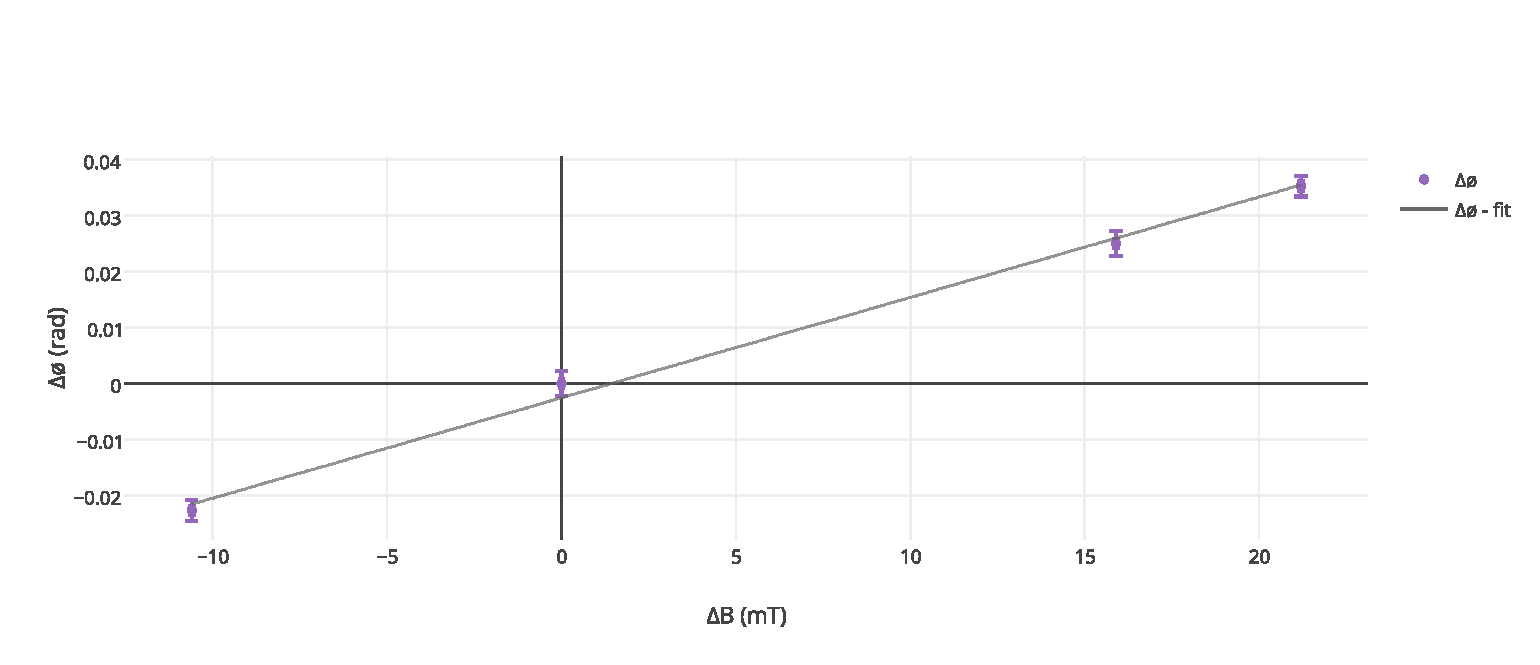
\includegraphics[width =6.3in]{verdet1.pdf}
\caption{\label{method2pic} The relative polarization shift for various magnetic fields. A linear was used to determine $\Delta \phi/\Delta B$.}
\end{figure}
}
\section{Discussion}

{We compared our values for the Verdet Constant with those found by colleagues performing the same experiment.  With Method 1, our colleagues found the value of the $V_{c}$ to be between 19 and 23 $\mathrm{~rad/T} \cdot \textrm{m}$.  Our value of $17.54 \pm 1.12 \mathrm{~rad/T} \cdot \textrm{m}$ is within this range for two standard deviations.  Still, we consider systematic errors present in our data which would have generated an inaccurate value using Method 1.  The most likely parameter which went into Equation 3 that could exhibit a systematic error is our calculation of $\partial \theta/\partial B$.  It is possible a systematic error was present in our measurement of the phase shift offset.  We remarked earlier that the 305\degree--340\degree regions of all four of our datasets were offset from the sinusoidal fit, due to what appears to be a systematic error in data collection.  In order to rectify this error, we had excluded those points from our curve fit. 

We now explore possible causes of this systematic error.  Angle values in the 305\degree--340\degree range were more difficult to set on the Faraday Rotator as they were partially obstructed by the solenoid.  Using the human eye to set these values and attempting to look beyond the solenoid may have resulted in a systematic error in the angle setting due to parallax.  What looked like 305\degree might have actually been 303\degree--307\degree due to this parallax effect.  (~another reason?~).  We masked data values in this range in order to eliminate data values rendered invalid due to systematic error but perhaps we might have included several points which appeared fine but were also subject to systematic error.  Perhaps we should have thrown out all points beyond the 305 \degree mark as they might have all been intrinsically shifted from the sinusoidal curve they should have followed.  Including incorrect data points in the fit which generated our phase offset which was critical for the calculation in Method 1 would have resulted in a systematically incorrect offset and thus incorrect value for the Verdet Constant.

Using Method 2, our colleagues found the $V_{c}$ to be between 19 and 21$\mathrm{~rad/T} \cdot \textrm{m}$.  Our $V_{c}$ using Method 2, $19.9 \pm 1.0 \mathrm{~rad/T} \cdot \textrm{m}$ is thus in good agreement with the values of our fellow researchers as it falls within that range, within error. Method 2 involved parameters which did not depend on the accuracy of the phase offset and sinusoidal fit and thus our systematic error did not affect the calculations from Method 2.  Our Verdet constant from Method 2 is thus the one to be reported as accurate.  It was in agreement with the values reported by our colleagues, as mentioned earlier.}

\section{Conclusion}
{\begin{enumerate}[(a)]
\item We were able to demonstrate Faraday Rotation for 3 different values of magnetic field.  As can be seen from the graphs, each plot of rotation angle vs. voltage has a different offset from the graph of rotation angle vs. voltage for a zero-field case.  We can conclude that the overall plane of polarization for incident light has been rotated due to its travel through a magnetic field.
\item We calculated the Verdet Constant using two different methods of calculation.  The first method gave us a constant of $19.9 \pm 1.0 \mathrm{~rad/T} \cdot \textrm{m}$, which is in good agreement with the values our colleagues calculated.  The second method was likely affected by a systematic error in our data recording and ended up being $17.54 \pm 1.12 \mathrm{~rad/T} \cdot \textrm{m}$, not within agreement of the values calculated by our colleagues.
\end{enumerate}}

\section{References}

\begin{thebibliography}{4}

\bibitem{optics} The Properties of Optical Glass.  Hans Back and Norbert Neuroth.  Springer Science $\&$ Business Media, 1998.

\bibitem{melissinos} Experiments in Modern Physics.  Adrian Constantin Melissinos and Jim Napolitano.  Gulf Professional Publishing, 2003

\bibitem{teachspin}Instructor's Guide to TeachSpin's FR1-A Apparatus.  Jonathan F. Reichert

\bibitem{expphysics}The Art of Experimental Physics.  Daryn W. Preston and Eric R. Dietz.  John Wiley  $\&$ Sons, Inc, 1991.

\bibitem{spin}Magneto-optical Faraday effect in spin-liquid candidates.  Jacob R. Colbert, H. Dennis Drew, and Patrick A. Lee.  Phys. Rev. B 90, 121105(R) – Published 12 September 2014



\end{thebibliography}


\end{document}
